\chapter{FPGA NES kártya ismertetése}
\label{sec:fpga-nes-board-summary}

A NES hardverének újragondolásából \aref{fig:PCB-blockdiagram}. ábrán látható blokkdiagramot készítettem, ez a nyomtatott huzalozott kártyák tervezésének első lépése. Már itt érdemes feltüntetni a különböző áramköri elemek közti kommunikációs utakat (busz típusokat), illetve ezek irányát. A diagram alapján elkezdődhet a különböző komponensek keresése, ezt követően át kell gondolnunk ezek fogyasztását és feszültség szintjeit, majd ezekből az adatokból már megtervezhető a kártya tápellátása is (a mi esetünkben már kiegészítettem ezzel a blokkdiagramot). 

\begin{figure}[H]
	\centering
	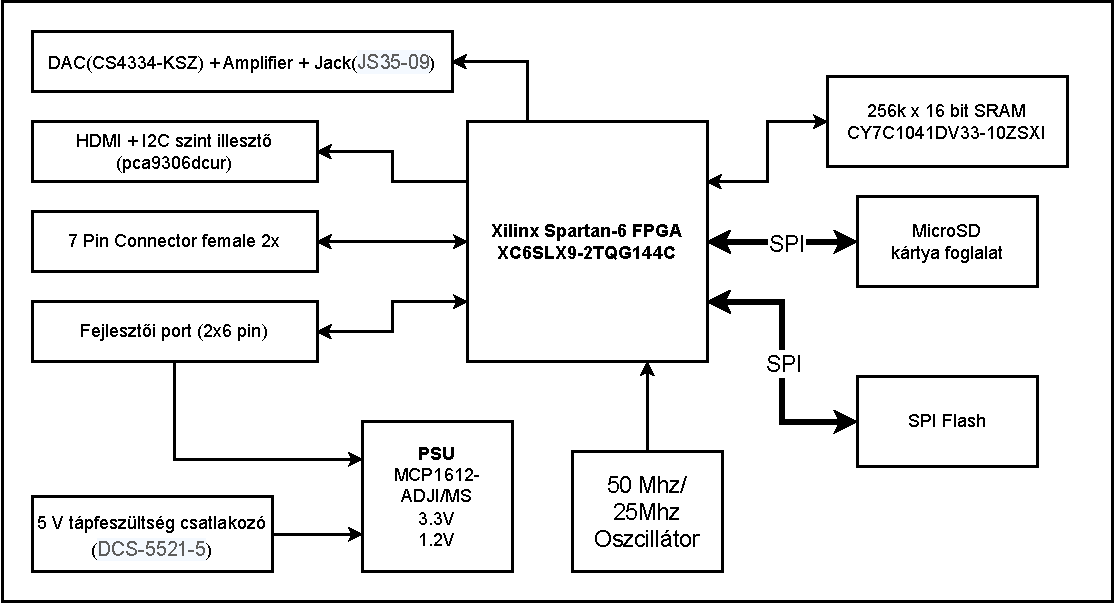
\includegraphics[width=150mm, keepaspectratio]{figures/NES-board-blockdiagram}
	\caption{NES kártya blokkdiagramja}
	\label{fig:PCB-blockdiagram}
\end{figure}

A komponensek közül az FPGA chip kiválasztása a legnehezebb. Ennek menete általában az, hogy megpróbáljuk felmérni az FPGA-val elvégzendő feladat hardveres méretét és ez alapján választunk megfelelő erőforrásokkal ellátott chip-et. A mi esetünkben az egyik legkomplexebb elem a 6502-es 8 bites processzor, amely méretét az OpenCores weboldalon \cite{OpenCore} található nyílt forráskódú hardvertervek alapján 1000 LUT-ra becsülhetjük. A NES működéséhez három fő komponens kell (CPU, APU, PPU), ezek méretét egyesével felülbecsülhetjük a legkomplexebb alkatrész méretével, így összesen 3000 LUT-ot kapunk. Ehhez még érdemes a VGA jel előállítását (TMDS jel kódolása), illetve az audió jel kezelését még hozzászámolni, erre is jó felső becslés az 1000 LUT. Végül még érdemes tartalékkal is számolni, ezért egy 5000-6000 LUT-al rendelkező FPGA chip valószínűleg elég nagy ahhoz, hogy a teljes projekt elférjen benne. Fontos kritérium még, hogy DCM-el és PLL-el rendelkezzen a chip az egyedi órajelek előállítása érdekében (például a 250 MHz a TMDS bitek kiadásához), ezen kívül még blokk RAM-ra is szükség lesz, legalább akkorára, mint a NES hardverének belső memóriája.  

%todo kell e ide a konzulens hivatkozása Szerencsére a konzulensem jóvoltából, szert tettem
A feladat megvalósításához egy Spartan-6-os Xilinx FPGA állt a rendelkezésemre, amely megfelel a fent említett összes elvárásnak. Ez a chip nagyban meggyorsította a nyáktervezés menetét is, mivel az egyetemi Spartan-6-os fejlesztő kártyák fő komponense is ez az FPGA volt \cite{spatan6}. Ezt a fejlesztő kártyát vettem alapul a NES kártyám fejlesztő portjának kialakítása, az SPI flash bekötése, illetve a tápvonalak kialakítása során is. 
	
A kártyán az alábbi komponensek találhatóak:

\begin{itemize}
	\item \emph{FPGA:} Xilinx XC6SLX9-2TQG144C típusú Spartan-6-os FPGA, amely lehetővé teszi az összetettebb logikák és
	a mikroprocesszoros rendszerek megvalósítását. Az eszköz főbb jellemzői:
		\begin{itemize}
			\item 5720 darab 6 bemenetű LUT és 11440 darab flip-flop
			\item 32 darab 18 kilobites blokk RAM
			\item 16 darab DSP48A1 blokk (elő összeadó, 18x18 bites előjeles szorzó és akkumulátor)
			\item 4 darab DCM (Digital Clock Manager) és 2 darab PLL (Phase Locked Loop) modul
		\end{itemize} 
	\item \emph{Memóriák a program és az adatok tárolására:}
		\begin{itemize}
			\item Egy 256kx16 bites (512 kB), 10 ns-os aszinkron SRAM (Cypress CY7C1041DV33-10ZSXI)
			\item Egy 32 Megabites SPI buszos soros flash memória (Atmel AT25DF321A), amely
			konfigurációs memóriaként is szolgál az FPGA számára
		\end{itemize}
	\item \emph{Egy MicroSD memóriakártya foglalat:}
		\begin{itemize}
			\item Teljes MicroSD kártya protokoll
			\item Egyszerű SPI protokoll
		\end{itemize}
	\item \emph{Beviteli eszközök:}
		\begin{itemize}
			\item Két eredeti 7 lábas NES (GamePAD) kontroller csatlakozók
			\item Reset és PROG gombok
		\end{itemize}	
	\item \emph{Képfeldolgozás:}
		\begin{itemize}
			\item HDMI csatlakozó 
			\item I2C szint illesztő (PCA9306DCUR típusú), megjelenítő EDID ROM-jának ki olvasásához 
		\end{itemize}
	\item \emph{Audio:}
		\begin{itemize}
			\item Digitális-analóg átalakító (DAC), CS4334-KSZ típusú  
			\item 100 mW-os TS486IST típusú erősítő (fülhallgatókhoz)
			\item CUI SJ1-3553NG 3,5mm Jack csatlakozó
		\end{itemize}
	\item \emph{Tápegységek:} MCP1612-ADJI/MS típusú szinkron buck konverterek
	\item \emph{Egy 50 MHz-es oszcillátor} 
	\item \emph{Csatlakozó a LOGSYS fejlesztői kábel számára} 
\end{itemize}
	
\section{Tápellátás}
	
	A tápellátás kialakítása a Logsys Spartan-6-os fejlesztői kártyáéhoz hasonló \cite{spatan6}. A NES kártya 5 V-os tápfeszültségről működik. Ezt a tápellátást vagy a fejlesztő kábelről kapja az eszköz, vagy egy külső 5 V-os forrásból. A külső egyenfeszültségű forrást Schottky dióda védi, illetve a kártyán elhelyeztem egy tápellátást jelző zöld LED-et is (PWR). 
	
	Az 5 V-os forrást két azonos típusú step down (buck) konverterrel 3,3 V-ra és 1,2 V-ra konvertálom. Alapvetően az FPGA működéséhez kell a két feszültségszint. A 3,3 V az I/O vonalakért, a DCM, a PLL és a konfigurációért felelős, míg az 1,2 V pedig az FPGA belső magjának kell. Ezt a két tápvonalat az FPGA dokumentációja alapján (a táp lábaihoz közel) elláttam a megfelelő mennyiségű csatoló (coupling) és hidegítő (bulk) kapacitásokkal a stabil működés érdekében. A 3,3 V-ot a kártyán található többi alkatrész is használja (SRAM, MicroSDkártya, kontrollerek, a fejlesztő kábel is megkapja, mint JTAG referencia feszültség, stb.). A kártya a HDMI csatlakozó, a DAC és az erősítő komponensek esetén a tápellátás 5 V-ját használja fel. A tápellátás kapcsolási rajzát \aref{sec:PSU}. függelékben láthatjuk. 
	 
\section{Órajel források}
	
	A NES kártyán a Logsys fejlesztő kártyához hasonlóan egy 50 MHz-es oszcillátort helyeztem el. Az FPGA, vagy a fejlesztő portról érkező CLK-tól kapja az órajelét, vagy az 50 MHz-es oszcillátorról. Ahhoz, hogy az FPGA használhassa ezeket az órajeleket, egy-egy órajel bemeneti lábára (GCLK) kellett ezeket bekötni. Az oszcillátor segéd áramkörét \aref{sec:OSC-JTAG}. függelékben láthatjuk. % és órajel források bekötését pedig \aref{tab:FPGA-OSCpin} táblázatban olvashatjuk.
	
%	\begin{table}[H]
%		\footnotesize
%		\centering
%		\begin{tabular}{|l|l|}
%			\hline
%			\rowcolor[HTML]{C0C0C0} 
%			\multicolumn{1}{|c|}{\cellcolor[HTML]{C0C0C0}{\color[HTML]{333333} \textbf{Órajel forrás}}} & \multicolumn{1}{c|}{\cellcolor[HTML]{C0C0C0}{\color[HTML]{333333} \textbf{FPGA láb}}} \\ \hline
%			50 MHz-es oszcillátor                                                                       & P85                                                                                   \\ \hline
%			Fejlesztői port CLK vonala                                                                  & P95                                                                                   \\ \hline
%		\end{tabular}
%		\caption{FPGA órajel forrásainak bekötése}
%		\label{tab:FPGA-OSCpin}
%	\end{table}
	
\section{Memória - SRAM}
	
	A választott aszinkron SRAM mérete 256kx16 bit (512 kilobájt). Ez a méret megfelel \aref{sec:Game-store}. fejezetben tárgyalt játék méreteknek (csak egy NES játék nem fog beleférni ebbe a RAM-ba). A választott memória előnye, hogy 10 ns elérési idejű aszinkron, statikus RAM, egyszerű kezeléssel. Ez azért jelent előnyt a konzol hardveres emulálása szempontjából, mert nem fogja ennek működését befolyásolni a memória elérési idő (a későbbiekben az elérést igazíthatjuk az általunk választott időzítéshez). DRAM esetén sokkal több időzítési paraméterrel kell számolni, ez jóval megnehezítené egy időzítés kritikus hardver létrehozását.
	
	Az SRAM 18 bites címmel rendelkezik, ezzel az adataink 2 bájtosával címezhetőek (összesen 256 kilobájt cím). A RAM-ból kiolvasott, illetve beírandó adatokat pedig a 16 bites adatvonalak segítségével érhetjük el. Az SRAM vezérlésétől függően kiolvasható vagy írható egyszerre mind a 16 bit, de van bájtos elérési mód is.
	
	Az SRAM szabványos vezérlési felülettel rendelkezik. A következő vezérlőjelek segítségével tudjuk irányítani (ezek mindegyike negált logikájú): chip engedélyezés CSn, írás engedélyezése WEn, olvasás engedélyezés OEn, alsó bájt engedélyezés LBn, végül pedig a felső bájt engedélyezés UBn. A memória olvasási és írási idő diagramjait \acite{sram} adatlapban olvashatjuk, a kiegészítő áramkörét pedig \aref{sec:SRAM-SPI-Flash}. függelékben láthatjuk.     
	
%	\begin{table}[H]
%		\footnotesize
%		\centering
%		\begin{tabular}{|lccccccccc|}
%			\hline
%			\rowcolor[HTML]{C0C0C0} 
%			\multicolumn{10}{|l|}{\cellcolor[HTML]{C0C0C0}\textbf{Címbusz}}                                                                                                                                                                                                                                                                                                                                                                                                                                                                                                                                                                                                                                      \\ \hline
%			\rowcolor[HTML]{EFEFEF} 
%			\multicolumn{1}{|l|}{\cellcolor[HTML]{EFEFEF}SRAM}                            & \multicolumn{1}{c|}{\cellcolor[HTML]{EFEFEF}A0}                         & \multicolumn{1}{c|}{\cellcolor[HTML]{EFEFEF}A1}                         & \multicolumn{1}{c|}{\cellcolor[HTML]{EFEFEF}A2}                         & \multicolumn{1}{c|}{\cellcolor[HTML]{EFEFEF}A3}                         & \multicolumn{1}{c|}{\cellcolor[HTML]{EFEFEF}A4}                         & \multicolumn{1}{c|}{\cellcolor[HTML]{EFEFEF}A5}                         & \multicolumn{1}{c|}{\cellcolor[HTML]{EFEFEF}A6}                         & \multicolumn{1}{c|}{\cellcolor[HTML]{EFEFEF}A7}                         & A8   \\ \hline
%			\rowcolor[HTML]{EFEFEF} 
%			\multicolumn{1}{|l|}{\cellcolor[HTML]{EFEFEF}{\color[HTML]{333333} FPGA láb}} & \multicolumn{1}{c|}{\cellcolor[HTML]{EFEFEF}{\color[HTML]{333333} P47}} & \multicolumn{1}{c|}{\cellcolor[HTML]{EFEFEF}{\color[HTML]{333333} P46}} & \multicolumn{1}{c|}{\cellcolor[HTML]{EFEFEF}{\color[HTML]{333333} P45}} & \multicolumn{1}{c|}{\cellcolor[HTML]{EFEFEF}{\color[HTML]{333333} P44}} & \multicolumn{1}{c|}{\cellcolor[HTML]{EFEFEF}{\color[HTML]{333333} P43}} & \multicolumn{1}{c|}{\cellcolor[HTML]{EFEFEF}{\color[HTML]{333333} P34}} & \multicolumn{1}{c|}{\cellcolor[HTML]{EFEFEF}{\color[HTML]{333333} P33}} & \multicolumn{1}{c|}{\cellcolor[HTML]{EFEFEF}{\color[HTML]{333333} P32}} & P30  \\ \hline
%			\multicolumn{1}{|l|}{SRAM}                                                    & \multicolumn{1}{c|}{A9}                                                 & \multicolumn{1}{c|}{A10}                                                & \multicolumn{1}{c|}{A11}                                                & \multicolumn{1}{c|}{A12}                                                & \multicolumn{1}{c|}{A13}                                                & \multicolumn{1}{c|}{A14}                                                & \multicolumn{1}{c|}{A15}                                                & \multicolumn{1}{c|}{A16}                                                & A17  \\ \hline
%			\multicolumn{1}{|l|}{FPGA láb}                                                & \multicolumn{1}{c|}{P29}                                                & \multicolumn{1}{c|}{P7}                                                 & \multicolumn{1}{c|}{P6}                                                 & \multicolumn{1}{c|}{P5}                                                 & \multicolumn{1}{c|}{P2}                                                 & \multicolumn{1}{c|}{P1}                                                 & \multicolumn{1}{c|}{P139}                                               & \multicolumn{1}{c|}{P138}                                               & P137 \\ \hline
%		\end{tabular}
%		\caption{SRAM memória címbusz bekötése}
%		\label{tab:FPGA-MEM-SRAMpin}
%	\end{table}
%		
%	\begin{table}[H]
%		\footnotesize
%		\centering
%		\begin{tabular}{|lcccccccc|}
%			\hline
%			\rowcolor[HTML]{C0C0C0} 
%			\multicolumn{9}{|l|}{\cellcolor[HTML]{C0C0C0}\textbf{Adatbusz}}                                                                                                                                                                                                                                                                                                                                                                                                                                                                                                                                                                                  \\ \hline
%			\rowcolor[HTML]{EFEFEF} 
%			\multicolumn{1}{|l|}{\cellcolor[HTML]{EFEFEF}SRAM}                            & \multicolumn{1}{c|}{\cellcolor[HTML]{EFEFEF}D0}                         & \multicolumn{1}{c|}{\cellcolor[HTML]{EFEFEF}D1}                         & \multicolumn{1}{c|}{\cellcolor[HTML]{EFEFEF}D2}                         & \multicolumn{1}{c|}{\cellcolor[HTML]{EFEFEF}D3}                         & \multicolumn{1}{c|}{\cellcolor[HTML]{EFEFEF}D4}                         & \multicolumn{1}{c|}{\cellcolor[HTML]{EFEFEF}D5}                         & \multicolumn{1}{c|}{\cellcolor[HTML]{EFEFEF}D6}                         & D7                         \\ \hline
%			\rowcolor[HTML]{EFEFEF} 
%			\multicolumn{1}{|l|}{\cellcolor[HTML]{EFEFEF}{\color[HTML]{333333} FPGA láb}} & \multicolumn{1}{c|}{\cellcolor[HTML]{EFEFEF}{\color[HTML]{333333} P40}} & \multicolumn{1}{c|}{\cellcolor[HTML]{EFEFEF}{\color[HTML]{333333} P17}} & \multicolumn{1}{c|}{\cellcolor[HTML]{EFEFEF}{\color[HTML]{333333} P21}} & \multicolumn{1}{c|}{\cellcolor[HTML]{EFEFEF}{\color[HTML]{333333} P22}} & \multicolumn{1}{c|}{\cellcolor[HTML]{EFEFEF}{\color[HTML]{333333} P23}} & \multicolumn{1}{c|}{\cellcolor[HTML]{EFEFEF}{\color[HTML]{333333} P24}} & \multicolumn{1}{c|}{\cellcolor[HTML]{EFEFEF}{\color[HTML]{333333} P26}} & {\color[HTML]{333333} P27} \\ \hline
%			\multicolumn{1}{|l|}{SRAM}                                                    & \multicolumn{1}{c|}{D8}                                                 & \multicolumn{1}{c|}{D9}                                                 & \multicolumn{1}{c|}{D10}                                                & \multicolumn{1}{c|}{D11}                                                & \multicolumn{1}{c|}{D12}                                                & \multicolumn{1}{c|}{D13}                                                & \multicolumn{1}{c|}{D14}                                                & D15                        \\ \hline
%			\multicolumn{1}{|l|}{FPGA láb}                                                & \multicolumn{1}{c|}{P8}                                                 & \multicolumn{1}{c|}{P9}                                                 & \multicolumn{1}{c|}{P10}                                                & \multicolumn{1}{c|}{P11}                                                & \multicolumn{1}{c|}{P12}                                                & \multicolumn{1}{c|}{P14}                                                & \multicolumn{1}{c|}{P15}                                                & P16                        \\ \hline
%		\end{tabular}
%		\caption{SRAM memória adatbusz bekötése}
%		\label{tab:FPGA-DATA-SRAMpin}
%	\end{table}
%
%	\begin{table}[H]
%		\footnotesize
%		\centering
%		\begin{tabular}{|llllcc|}
%			\hline
%			\multicolumn{6}{|l|}{\cellcolor[HTML]{C0C0C0}\textbf{Vezérlő jelek}}                                                                                \\ \hline
%			\multicolumn{1}{|l|}{SRAM}     & \multicolumn{1}{l|}{CSn} & \multicolumn{1}{l|}{WEn} & \multicolumn{1}{l|}{OEn}  & \multicolumn{1}{c|}{LBn}  & UBn  \\ \hline
%			\multicolumn{1}{|l|}{FPGA láb} & \multicolumn{1}{l|}{P41} & \multicolumn{1}{l|}{P35} & \multicolumn{1}{l|}{P140} & \multicolumn{1}{c|}{P142} & P141 \\ \hline
%		\end{tabular}
%		\caption{SRAM memória vezérlő jelek bekötése}
%		\label{tab:FPGA-CONTROL-SRAMpin}
%	\end{table} 
	
\section{Digital Analog Converter és erősítő}
	
	A NES kártya egyetlen analóg alkatrészekre támaszkodó része a DAC-ot követő erősítő áramkör, ennek részletes megértéséhez tekintsük meg \aref{fig:DAC-AMP-JACK}. ábrát, amely \aref{sec:DAC-controllers}. függelékből lett kiemelve.
	
	A DAC komponenst egy 100 MHz-en 600 $\Omega$-os Ferrite Bead-el védem az esetleges 5 V-os tápvonalról beszűrődő zajokkal szemben. Ide szűrési okokból tantál és kerámia kondenzátorokat is helyeztem. Az alkatrész az FPGA által előállított mono digitális "hang" jelet alakítja át és adja ki mind a két kimenetén. Ezek az analóg jelek fognak az erősítést követően, a Jack csatlakozó bal és jobb fülhöz menő lábára csatlakozni. 
	
	A DAC két kimenetét, egy-egy 3,3 uF-os csatoló kondenzátorral választom el az analóg résztől. Az áramkörben található C38, C39-es kondenzátorok és R27, R28-as ellenállások egy aluláteresztő szűrőt valósítanak meg. A kondenzátorok értékét, pedig a következő képlet alapján határoztam meg (az ellenállások értéke kötött volt az erősítő miatt):
	
	\begin{align}	
		C = \frac{R + 560 \Omega}{4} *\pi * Fs * (R * 560 \Omega)
	\end{align} 
	
	Itt $Fs$ az általunk választott audió jel frekvenciája, az 560 $\Omega$ pedig a soros ellenállás értéke. Ezek alapján a két kondenzátorom értéke 3,3 nF vagy 2,7 nF lehet, mivel így 48 kHz-hez közeli értéket kapunk a frekvenciára. Az összes kerámia kondenzátornak, amely az analóg áramkör része NP0 (vagy C0G) dielektrikummal kell rendelkeznie, mivel ezeknek nincs piezoelektromos tulajdonságuk.   
	
	\begin{figure}[H]
		\centering
		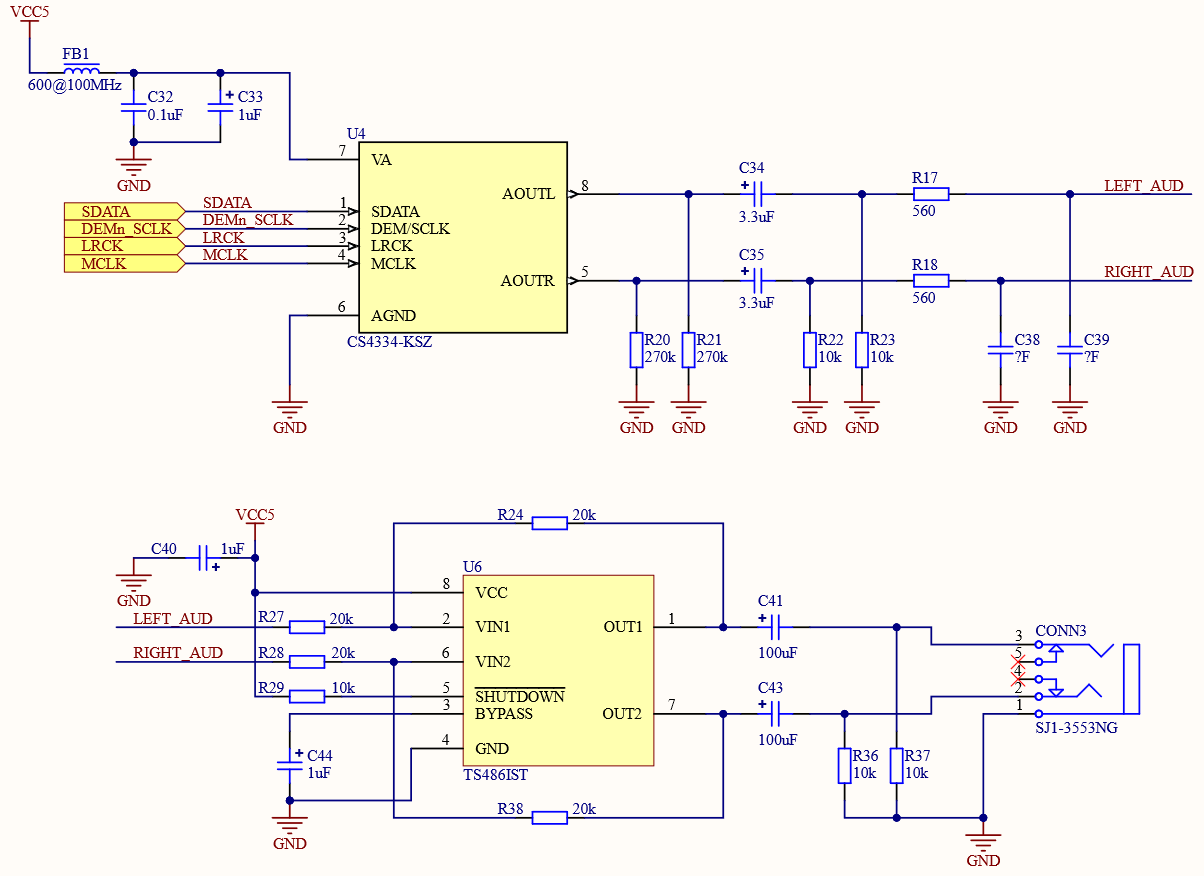
\includegraphics[width=150mm, keepaspectratio]{figures/DAC-AMP-JACK}
		\caption{NES audió jelért felelős áramkörök}
		\label{fig:DAC-AMP-JACK}
	\end{figure}
	
	Az erősítő komponensnek egy fázisfordító erősítőt választottam, amely erősítése az R27 és R24, illetve az R28 és R38 ellenállásokkal módosítható a következő képletek alapján:
	
	\begin{align}	
		Gain_{LINEAR} = -\frac{RFEED}{RIN}
	\end{align} 
	
	\begin{align}	
		Gain_{dB} = 20 * lg(\frac{RFEED}{RIN})
	\end{align}
 
	Az áramkörben jelenleg nem állítottam be erősítést, az RFEED és RIN ellenállások értékét 20 k$\Omega$-nak határoztam meg. Ez természetesen a hardveres tesztelés során cserélhető és állítható.	
	
\section{HDMI és I2C szint illesztő}
	\label{sec:HMI-I2C}
	
	A NES nyomtatott huzalozott kártyáján elhelyeztem egy HDMI csatlakozót és a körülötte elhelyezkedő áramkör segítségével felkészítettem TMDS jelek kiadására. A teljes áramkör kapcsolási rajzát \aref{sec:HDMI-MicroSDcard}. függelékben láthatjuk.
	
	A jövőbeli fejlesztések miatt elhelyeztem a nyákon még egy I2C jelszint illesztőt is, hogy ennek segítségével a csatlakoztatott eszköz EDID ROM-ját ki tudjam olvasni. Ebből megállapítható, hogy képes-e audió adatok vételére a TV vagy monitor, így a kártya támogatja ezen eszközök beépített hangszóróit is. 
	
	Az alábbi ábrákon láthatjuk egy HDMI anya aljzat pin és láb kiosztását:   
	
	\begin{figure}[H]
	\begin{minipage}[]{\textwidth}
		\begin{minipage}[b]{0.39\textwidth}
			\centering
			\includegraphics[width=55mm, keepaspectratio]{figures/hdmi-Pinout}
			\captionof{figure}{aljzat anya \cite{HDMI}}
			\label{fig:HDMI-pinout}
		\end{minipage}
		\hfill
		\begin{minipage}[b]{0.59\textwidth}
			\footnotesize
			\centering
			\begin{tabular}{|l|c|l|c|}
				\hline
				\rowcolor[HTML]{C0C0C0} 
				\textbf{Funkció}  & \multicolumn{1}{l|}{\cellcolor[HTML]{C0C0C0}{\color[HTML]{333333} \textbf{Láb}}} & \textbf{Funkció}  & \multicolumn{1}{l|}{\cellcolor[HTML]{C0C0C0}{\color[HTML]{333333} \textbf{Láb}}} \\ \hline
				TMDS Data2+       & 1                                                                                & TMDS Clock Shield & 11                                                                               \\ \hline
				TMDS Data2 Shield & 2                                                                                & TMDS Clock-       & 12                                                                               \\ \hline
				TMDS Data-        & 3                                                                                & CEC               & 13                                                                               \\ \hline
				TMDS Data1+       & 4                                                                                & Reserved          & 14                                                                               \\ \hline
				TMDS Data1 Shield & 5                                                                                & SCL               & 15                                                                               \\ \hline
				TMDS Data1-       & 6                                                                                & SDA               & 16                                                                               \\ \hline
				TMDS Data0+       & 7                                                                                & DDC/CEC Ground    & 17                                                                               \\ \hline
				TMDS Data0 Shield & 8                                                                                & +5 V Power        & 18                                                                               \\ \hline
				TMDS Data0-       & 9                                                                                & Hot Plug Detected & 19                                                                               \\ \hline
				TMDS Clock+       & 10                                                                               &                   & \multicolumn{1}{l|}{}                                                            \\ \hline
			\end{tabular}
			\captionof{table}{HDMI lábkiosztás}
			\label{tab:HDMI-pinout}
		\end{minipage}
	\end{minipage}
	\end{figure} 
	
	Mivel az FPGA nem minden I/O láb pára képes differenciális jelek küldésére, ezért figyelni kell, hogy a csatlakozót az FPGA melyik oldalához közel helyezem el. A HDMI szabvány a differenciális vonalakra 100 $\Omega$-os differenciális impedanciát ír elő (15 \%-os toleranciával), ezért érdemes ezeket a vezetékeket minél rövidebben huzalozni (FPGA bekötési oldalhoz közel). 
	
	Az alkatrészeim védelmére a HDMI 5 V-os tápellátását egy 100 mA-es biztosítékon (poli fuse) vezettem keresztül, ez túláram esetén véd. A csatlakozó fém burkolatát egy 1 M$\Omega$-os ellenállással és egy 1 nF-os (1 kV-os) kapacitással földeltem, ez HDMI kimenetek esetén ideális. 
	
\section{A kártya bemenetei}
	
	A NES nyomtatott huzalozott kártyáját az eredeti játékkonzol kontroller csatlakozóival láttam el. Az eredeti kontroller a NES 5 V-járól működik, viszont a benne található párhuzamos-soros átalakító (shiftregiszter) az adatlapja alapján 3,3 V-ról is működik. Ez azért fontos, mert így nem kell extra jelszint illesztő IC a kártyára, működtethetem az adat fogadást és az órajel küldést az FPGA I/O lábairól (3,3 V).
	
	Ennek a kontrollernek egyedi hét lábas anya csatlakozója van, amit \aref{fig:7PIN-Port}. ábrán láthatunk.   
	
	\begin{figure}[H]
		\centering
		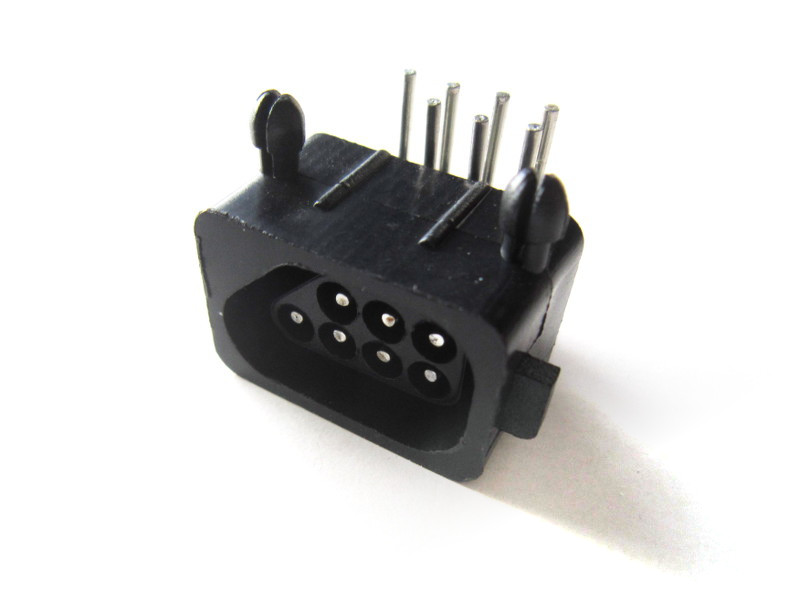
\includegraphics[width=80mm, keepaspectratio]{figures/7pin-connector} %110
		\caption{NES kontroller csatlakozó \cite{NES_controller}}
		\label{fig:7PIN-Port}
	\end{figure}
	
	Ebből a hét lábból kettőnek csak rögzítési szerepe van, kettő a tápellátásért felelős és a maradék három lábon keresztül történik a kontrollerben található regiszter olvasása, vezérlése és a működési órajel küldése. A kártyára ebből a csatlakozóból kettőt helyeztem el a kooperatív játékok végett. A kontroller portok kapcsolási rajzát \aref{sec:DAC-controllers}. függelékben láthatjuk.
	
	A nyákon négy gomb is helyet kapott: az első az FPGA és ezáltal a NES reset gombja (RST), a második az FPGA újrakonfigurálását elindító nyomógomb (PROG), a harmadik és negyedik pedig a hangerő növelő és csökkentő gombok. Az gombok pergés mentesítéséért az FPGA felelős. Ezek mindegyikét \aref{sec:OSC-JTAG}. függelékben láthatjuk. 
	
\section{MicroSD kártya}
	
	A MicroSD kártya csatlakozót teljes interfésszel tudtam implementálni, mivel az FPGA-nak még sok szabad I/O lába maradt. Ez azt jelenti, hogy teljes SD kártya protokollt is megtudok valósítani a NES fejlesztő kártyán az egyszerűbb soros SPI kommunikáció mellett. A MicroSD kártya segéd áramkörét \aref{sec:HDMI-MicroSDcard}. függelék kapcsolási rajzán láthatjuk. 
	
	Itt érdemes az áramkör ki-és bekapcsolásáért felelős P-MOSFET-es áramkört megnézni. Ez azért szükséges, mert a fent említett két protokoll közötti váltáshoz áramtalanítanunk kell az SD kártyát. A tápellátás elvétele mellett a felhúzó ellenállások tápellátását is elvesszük kikapcsolás során. Egyedül a CD kártya detektáló lábtól nem vesszük el, mivel ez csak azt jelzi, hogy van-e SD kártya a csatlakozóban (nem része a fent említett kommunikációs protokolloknak). Ezt a be- és kikapcsolási eseményt az FPGA egy I/O lábának segítségével vezéreljük.
	
	Az esetleges túllövések csökkentése érdekében elhelyeztem az SD kártya CLK lábára egy 33 $\Omega$-os soros ellenállást, ezt a PCB layout tervezése során a lehető legközelebb helyeztem el az FPGA-hoz.  
	
\section{FPGA konfigurációs módok}
	
	A NES kártyának is a LOGSYS Spartan-6 FPGA kártyához hasonló módon \cite{spatan6} két konfigurációs módja van. Az FPGA-t felprogramozhatjuk a fejlesztői porton található JTAG interfész segítségével, illetve felkonfigurálhatja saját magát a kártyán található soros flash memóriából is. A konfigurációs módok között egy rövidzár segítségével (jumper) válthatunk a LOGSYS-es kártyához hasonlóan. Ennek működését \aref{tab:FPGA-config}. táblázatban olvashatjuk, illetve \aref{sec:FPGA-BANKS}. függelékben láthatjuk.       
	
	\begin{table}[H]
		\footnotesize
		\centering
		\begin{tabular}{|c|c|l|}
			\hline
			\rowcolor[HTML]{C0C0C0} 
			\textbf{\begin{tabular}[c]{@{}c@{}}Jumper\\ állása\end{tabular}} & {\color[HTML]{333333} \textbf{\begin{tabular}[c]{@{}c@{}}Konfigurációs \\ mód\end{tabular}}} & \multicolumn{1}{c|}{\cellcolor[HTML]{C0C0C0}\textbf{Leírás}}                                                                                                                          \\ \hline
			\rowcolor[HTML]{FFFFFF} 
			\raisebox{-.5\height}{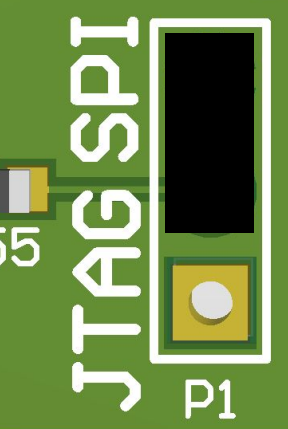
\includegraphics[width=10mm, keepaspectratio]{figures/SPI-jumper}}                                                                & JTAG                                                                                         & Az FPGA-t a JTAG interfészen keresztül kell felkonfigurálni.                                                                                                                           \\ \hline
			\rowcolor[HTML]{FFFFFF} 
			\raisebox{-.5\height}{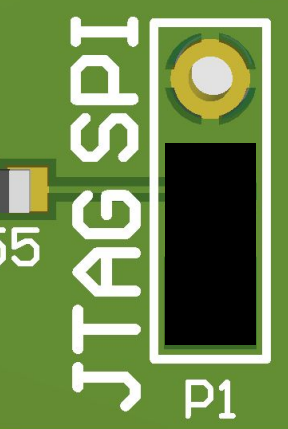
\includegraphics[width=10mm, keepaspectratio]{figures/JTAG-jumper}}                                                                & SPI                                                                                          & \begin{tabular}[c]{@{}l@{}}Az FPGA az SPI buszos soros flash memóriából konfigurálja \\ fel magát a tápfeszültség bekapcsolása vagy a PROG gomb \\ megnyomását követően.\end{tabular} \\ \hline
		\end{tabular}
		\caption{FPGA konfigurációs mód állítása}
		\label{tab:FPGA-config}
	\end{table}
	
\section{Soros flash memória}
	
	A NES kártyán egy Atmel AT25DF321A típusú, 32 Megabites, SPI busszal rendelkező soros flash memóriát helyeztem el. Ez a komponens az FPGA számára konfigurációs memóriaként szolgál (tehát a NES hardverének binárisát fogja tartalmazni). Ennek a komponensnek az elhelyezése, bekötése és ezáltal a működése is megegyezik a Logsys Spartan-6-os fejlesztői kártyán található flash-el \cite{spatan6}. A soros flash bekötését \aref{sec:SRAM-SPI-Flash}. függelékben láthatjuk.
	
	%TODO fix jumper heights if you have time
\section{LOGSYS fejlesztői port}
\label{sec:logsysport}
	
	A fejlesztői port kialakítása teljes mértékben megegyezik a Logsys fejlesztőkártyán található port-al, ennek köszönhetően az FPGA felprogramozása történhet a MIT tanszéken tervezett egyedi fejlesztőkábellel. Ennek részletes bemutatása \acite{spatan6}-os dokumentáció része. A fejlesztői port kialakítása \aref{sec:OSC-JTAG}. függelékben látható. Az FPGA sikeres felkonfigurálását egy zöld LED-el jelzem (DONE). %A fejlesztői port a következő elemekből áll:
	
%	\begin{enumerate}
%		\item JTAG interfész (vörös)
%		\item Soros SPI kommunikációs interfész (zöld)
%		\item 5 V-os egyenfeszültségű táp forrás (szürke)
%	\end{enumerate}
%	
%	\begin{figure}[H]
%		\begin{minipage}[]{\textwidth}
%			\begin{minipage}[b]{0.49\textwidth}
%				\centering
%				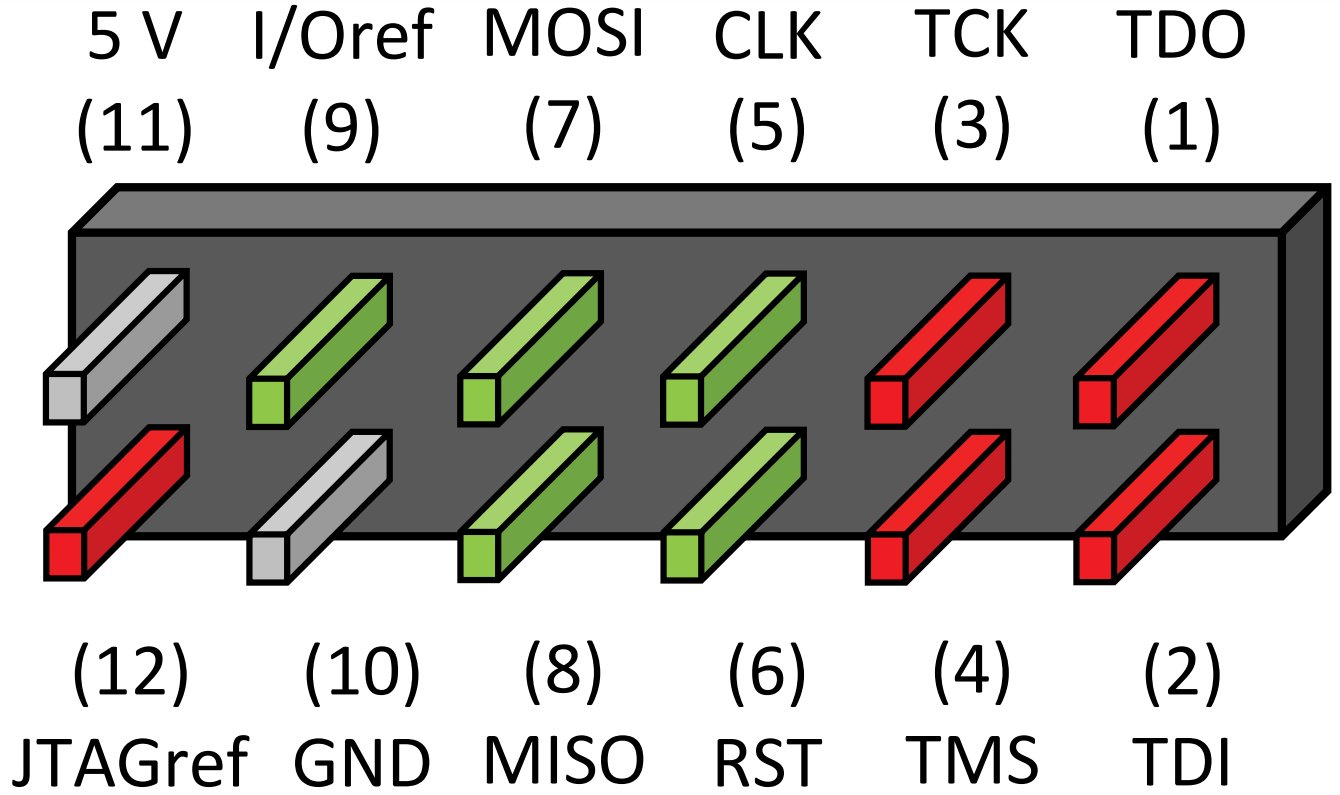
\includegraphics[width=50mm, keepaspectratio]{figures/DEV-port}
%				\captionof{figure}{Fejlesztői port kiosztása}
%				\label{fig:DEV-port}
%			\end{minipage}
%			\hfill
%			\begin{minipage}[b]{0.49\textwidth}
%				\footnotesize
%				\centering
%				\begin{tabular}{|l|l|l}
%					\cline{1-2}
%					\rowcolor[HTML]{C0C0C0} 
%					\multicolumn{1}{|c|}{\cellcolor[HTML]{C0C0C0}\textbf{jel}} & \multicolumn{1}{c|}{\cellcolor[HTML]{C0C0C0}{\color[HTML]{333333} \textbf{Irány}}} & \multicolumn{1}{c}{\cellcolor[HTML]{C0C0C0}\textbf{FPGA láb}} \\ \hline
%					\rowcolor[HTML]{FFFFFF} 
%					MOSI                                                       & bemenet                                                                            & \multicolumn{1}{l|}{\cellcolor[HTML]{FFFFFF}P104}             \\ \hline
%					\rowcolor[HTML]{FFFFFF} 
%					MISO                                                       & kimenet                                                                            & \multicolumn{1}{l|}{\cellcolor[HTML]{FFFFFF}P144}             \\ \hline
%					CLK                                                        & bemenet                                                                            & \multicolumn{1}{l|}{P95}                                      \\ \hline
%					RST                                                        & bemenet                                                                            & \multicolumn{1}{l|}{P94}                                      \\ \hline
%				\end{tabular}
%				\captionof{table}{Fejlesztői port bekötése}
%				\label{tab:DEV-pinout}
%			\end{minipage}
%		\end{minipage}
%	\end{figure} 		

\section{Nyomtatott áramköri terv}

A kapcsolási rajz megalkotását követően, a nyák tervezés következő fázisa a PCB rajzolat (layout) elkészítése. Itt természetesen figyelembe kell vennünk az eddig meghatározott célokat (lásd \ref{sec:Size}. fejezet), miszerint egy kompakt és hordozható eszközt tervezünk. Egy nyomtatott áramkör mérete nagyban függ a réteg felépítésétől, illetve a kiválasztott komponensek méretétől. Tehát minél több rétegből épül fel egy PCB és minél modernebb alkatrészeket használunk, annál nagyobb felületi alkatrész sűrűség érhető el. Természetesen ezekkel arányosan az ár is nő. Mivel először egy prototípust fejlesztek, ezért egy kompromisszumos megoldást kellett választanom.   
		
	\subsection{Réteg beállítások}
	
	A Logsys Spartan-6-os fejlesztőkártyán már láthattuk \cite{spatan6}, hogy a választott FPGA chip TQFP tokozása miatt kétrétegű nyákon behuzalozható. Az FPGA NES kártya tervezésekor ez egy fő szempont volt, mivel így érdekes mérnöki megoldásokat kellett alkalmaznom a táp bekötése során, illetve a kártya elkészítési költségét is csökkenteni tudtam.
	
	A prototípus kártyákat a JLCPCB nevű kínai cég gyártotta. Ahhoz, hogy az Altium tervező program képes legyen bonyolultabb számítások (differencial pair routing) és szimulációk készítésére, a réteg felépítést meg kell adnunk a PCB-nk számára. Ezt a kínai gyártó által szolgáltatott információk alapján \cite{jlcpcb} alakítottam ki, ez \aref{fig:Layer-stackup}. ábrán látható.    
	
	\begin{figure}[H]
		\centering
		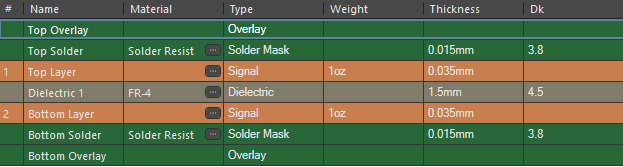
\includegraphics[width=150mm, keepaspectratio]{figures/Layer-stackup}
		\caption{Az FPGA NES kártya réteg beállításai}
		\label{fig:Layer-stackup}
	\end{figure}
	
	\subsection{Komponensek elhelyezése}
	
	A réteg beállításokat követően, a komponensek és segéd áramköreik elhelyezése következett. Ennek segítségével tudtam meghatározni végül, hogy az FPGA mely I/O bankjaihoz fogom vezetni a különböző komponensek kivezetéseit, illetve ez határozta meg a kártyám fizikai méreteit is. Az alkatrészek és segédáramköreik rajzolatát \aref{sec:NES-components}. függelékben láthatjuk, de a könnyebb áttekinthetőség érdekeben elkészítettem a következő ábrát is:
	
	\begin{figure}[H]
		\centering
		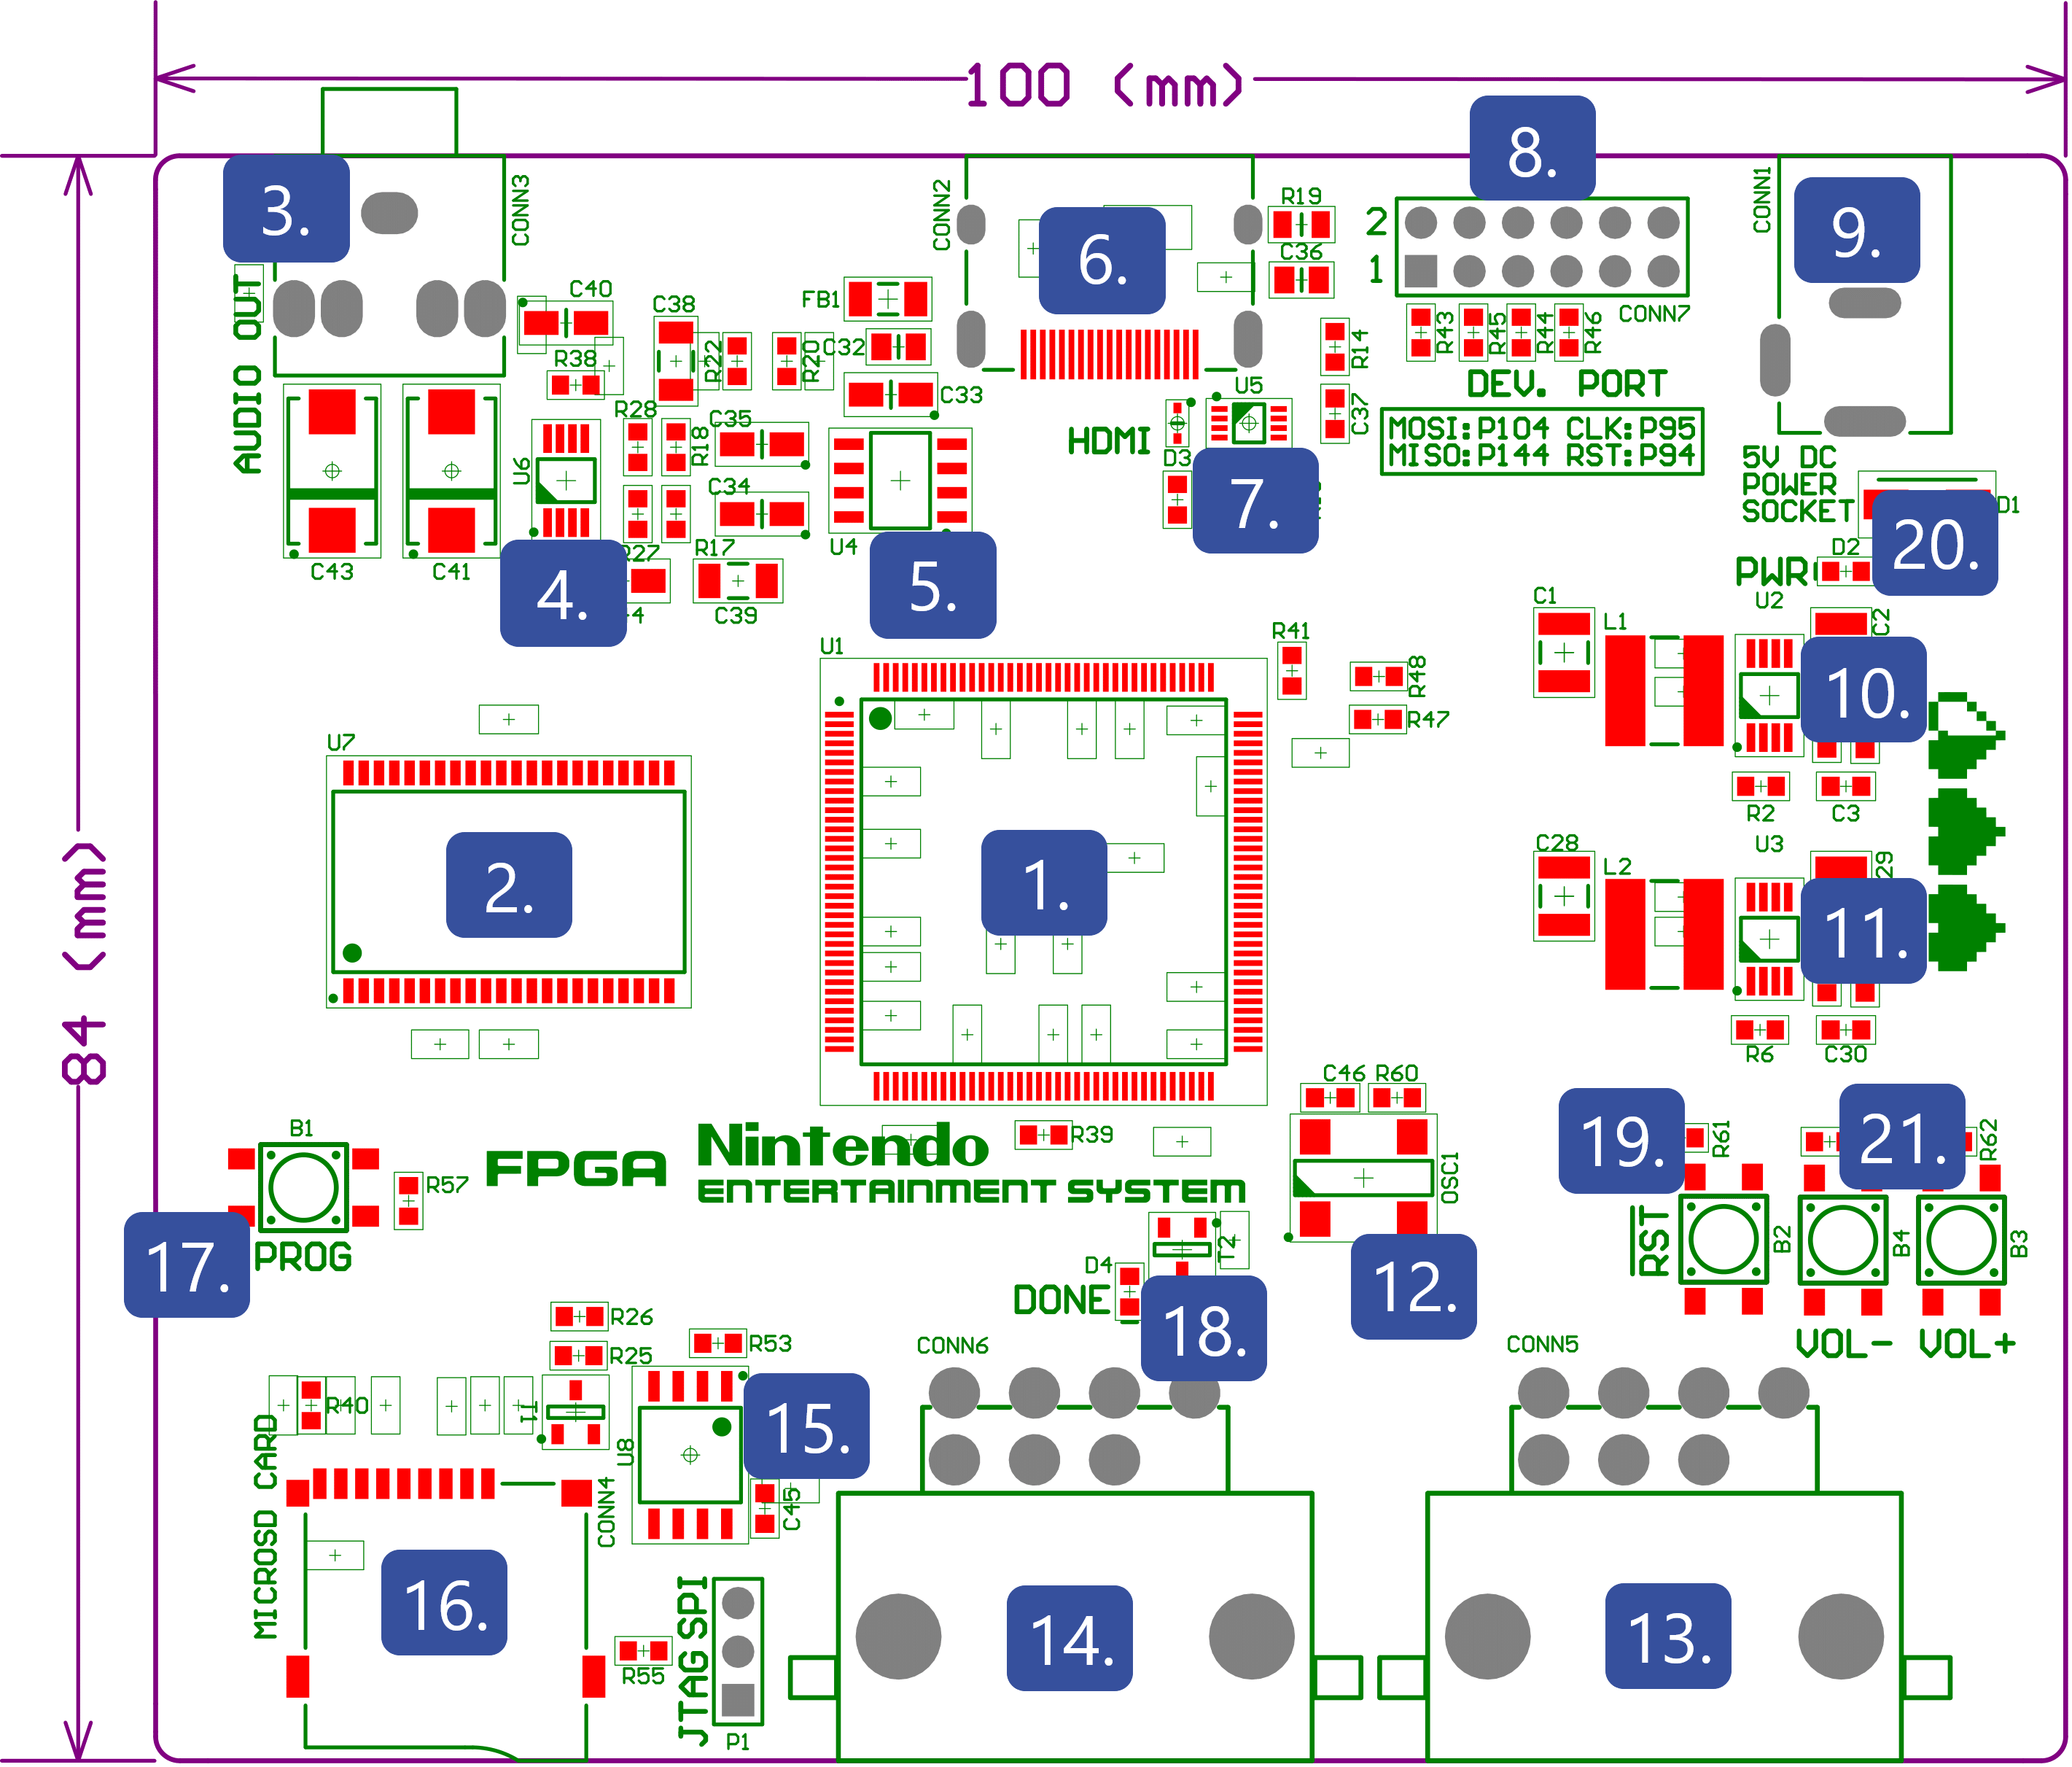
\includegraphics[width=135mm, keepaspectratio]{figures/components-top}
		\caption{A top layer alkatrész elhelyezési terve} 
		\label{fig:NES-components-top}
	\end{figure}
	
	FPGA NES kártya főbb alkotó komponensei:
	\begin{enumerate}
		\item Xilinx XC6SLX9-2TQG144C típusú FPGA
		\item 256kx16 bites (512 kB), 10 ns-os aszinkron SRAM (Cypress CY7C1041DV33-10ZSXI)
		\item 3,5 mm Jack csatlakozó (CUI SJ1-3553NG)
		\item 100 mW erősítő (TS486IST fülhallgatókhoz)
		\item Digital Analog Converter (DAC), (CS4334-KSZ)
		\item HDMI csatlakozó
		\item 2C szint illesztő (PCA9306DCUR)
		\item Csatlakozó a LOGSYS fejlesztői kábel számára
		\item 2,1 mm 12 V / 5 A DC táp csatlakozó (DC10A)
		\item 3,3 V feszültséget előállító tápegység
		\item 1,2 V feszültséget előállító tápegység
		\item 50 MHz-es oszcillátor 
		\item 7 lábú NES GamePAD kontroller csatlakozók anya aljzat 1
		\item 7 lábú NES GamePAD kontroller csatlakozók anya aljzat 2
		\item 32 Megabites SPI buszos soros flash (Atmel AT25DF321A)
		\item MicroSD kártya foglalat
		\item Az FPGA újrakonfigurálását indító gomb (PROG)
		\item Az FPGA sikeres felkonfigurálását jelző LED (DONE)
		\item Az FPGA kézi reset gombja (RSTn)
		\item A bekapcsolt tápfeszültséget jelző LED (PWR)
		\item A NES hangerő szabályzó gombjai (VOL-, VOL+)
	\end{enumerate}
	
	Mivel kézi forrasztással és hőfúvó segítségével fogjuk a kártyát összeállítani, ezért törekedtem arra, hogy az összes komponens (és ezek segédáramkörei) a felső (top) oldalon helyezkedjen el, illetve az alsó (bottom) csak azonos méretű elemek kerüljenek. Egyedül a HDMI csatlakozó biztosítéka került a hátoldalra, ami nem 0603-as méretű.
	
	Ezt követően a PCB alkatrészek bekötésével foglalkoztam. Itt az alsó és a felső réteget is jel/föld (signal/GND) rétegként alakítottam ki. Ez azt jelenti, hogy a jel vezetékeket és a tápvonalak bekötését követően az egész nyák felszínén föld kitöltést hoztam létre, így növelve a jelek integritását. Az alsó és a felső föld rétegeket, pedig via-k segítségével kötöttem össze (via stiching). A két rétegemet egyszerre \aref{sec:FPGA-nes-transparency}. függelékben láthatjuk, az itt használt réteg ábrázolási mód az Altium designer átlátszó 2D módja, amely betekintést enged a föld kitöltések alá. A felső réteg jelei és a komponensek pad-jei vörös színnel vannak jelölve, az alsó rétegé pedig kék színnel.
	
	\subsection{HDMI adatvonalainak bekötése}
	
	A HDMI vonalak kialakításáról már \aref{sec:HMI-I2C}. fejezet során olvashattunk. A réteg kialakítás során kétrétegű megvalósítást választottuk, de a PCB gyártó nem biztosít két réteg esetén impedancia kontrollálásra réteg felépítést, ezért a HDMI szabványban leírt 100 $\Omega$-os impedancia különbséget (15 \% os toleranciával) csak egy speciális differenciális pár bekötési típussal tudjuk biztosítani. Ez a típus a Dual Strip Coplanar Waweguide Grounded, ez azt jelenti, hogy differenciális pár bekötése mellett figyelnünk kell arra is, hogy a pár jobb és bal oldalán fix távolságra föld kitöltést helyezzünk el. Az itt található két réteg földjét az előre meghatározott távolságokon via fence-el látjuk el (ezt az elrendezést \aref{fig:coplanar}. ábrán láthatjuk). A viák közti maximális távolságot a következő képlettel számolhatjuk ki:
	
	\begin{align}
		\label{mat:via-distance}	
		S(via) = \frac{\lambda}{20} = \frac{c}{20 * f * \sqrt[]{\epsilon_r}}
	\end{align}   
	
	\Aref{mat:via-distance}. képletben található $\lambda$ a differenciális jelünk hullámhossza (a részletesebb képletben pedig: c a fény terjedési sebessége, f a jelünk frekvenciája, $\epsilon_r$ pedig az anyag relatív dielektromos állandója). A mi esetünkben ezen a vezeték páron 250 MHz-es jeleket fogunk küldeni, ennek hullámhossza körülbelül 1,151 m, ebből kiszámított két via közti maximális távolság 0,058 m (ennél természetesen választhatunk kisebb értéket is).
	
	\begin{figure}[H]
		\centering
		\includegraphics[width=90mm, keepaspectratio]{figures/coplanar}
		\caption{Dual Strip Coplanar Waweguide Grounded felépítése \cite{coplanar}} 
		\label{fig:coplanar}
	\end{figure}
	
	Az Altium Designer segítségével van lehetőségem a GND réteg és vezető pár közti távolság kiszámítására (később az ECAD szoftver ez alapján fogja elhelyezni a vezetékeket). Ezek a beállítások az alábbi ábrán láthatók:      
	
	\begin{figure}[H]
		\centering
		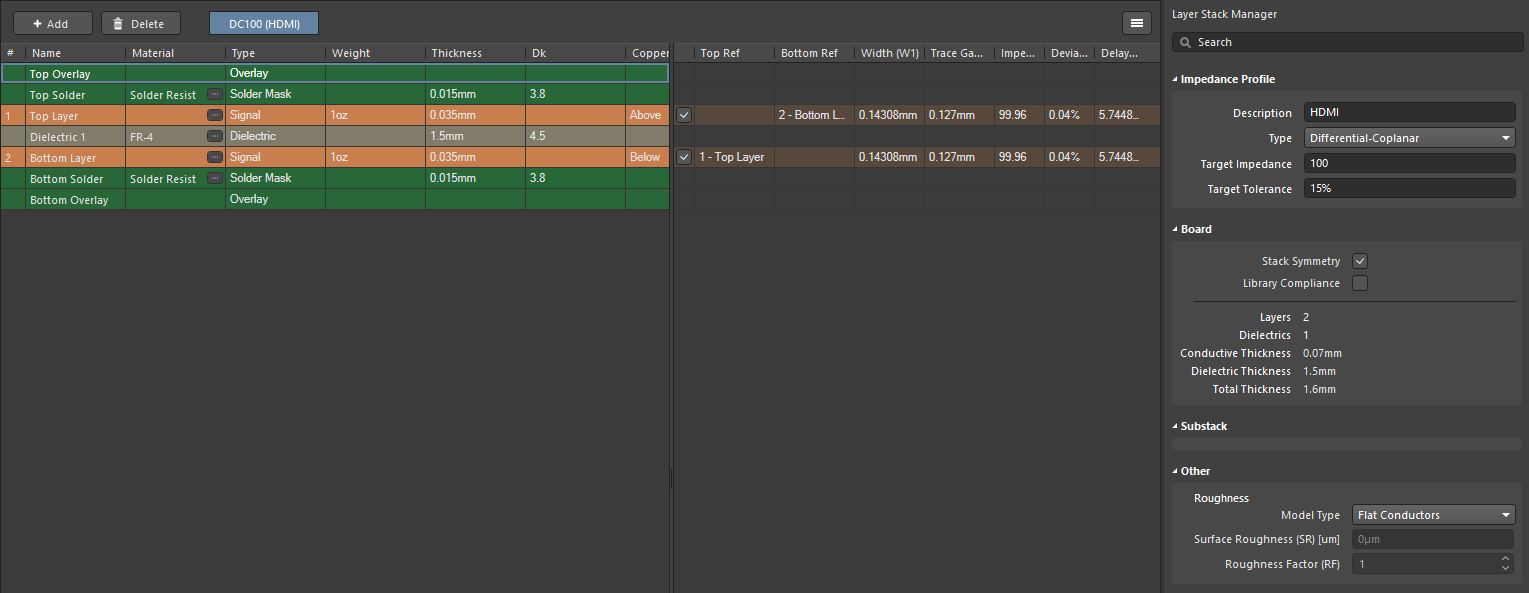
\includegraphics[width=150mm, keepaspectratio]{figures/Impedance-control}
		\caption{Coplanar differential pair routings Altium beállításai}
		\label{fig:Impedance-control}
	\end{figure}
	
	A FPGA NES kártya HDMI jeleinek bekötésére 2,75 mm-es via fence méretet választottam (körülbelül a fentebb kiszámolt érték 20-ad része). Ez részletesen \aref{fig:HDMI-Differencial-pair-routing}. ábrán látható, amely \aref{sec:FPGA-nes-transparency}. függelékből lett kiemelve.
	
	\begin{figure}[H]
	\centering
	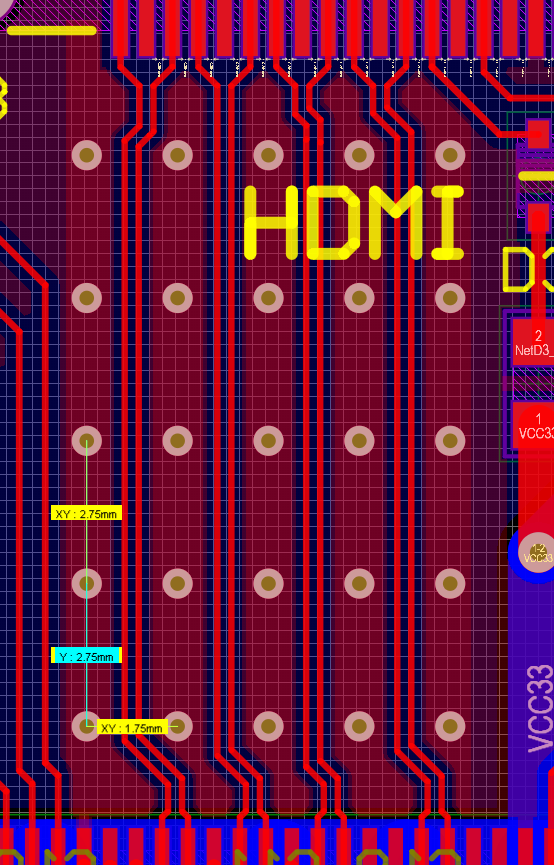
\includegraphics[width=90mm, keepaspectratio, angle=90]{figures/HDMI-Differencial-pair-routing}
	\caption{A HDMI adatvonalainak bekötése}
	\label{fig:HDMI-Differencial-pair-routing}
	\end{figure}
	
	\subsection{FPGA táp vonalak kialakítása}
	
	Ahhoz, hogy a Spartan-6-os FPGA chip-et két rétegen teljes mértékben ki tudjuk használni, egy speciális tápellátási módszerhez kellett folyamodnunk (Logsys-es fejlesztőkártya tápvonalai is hasonlóan vannak kialakítva). Ennek alapja az volt, hogy az alsó oldalról érkezik a 3,3 V és az 1,2 V is. A 3,3 V-ot az FPGA lábai alatt végigvezetjük (innen indul ki a többi 3,3 V-os komponens tápellátása is) egy helyen beengedve az 1,2 V-ot az FPGA belső magja számára. Ennek a rendszernek az előnye, hogy így az összes hidegítő (decoupling és bulk) kapacitás az FPGA alatt kaphat helyet, ezzel szabadon tartva a top réteget az FPGA I/O bankjainak és JTAG interfészének bekötésére.
	
	\begin{figure}[H]
		\centering
		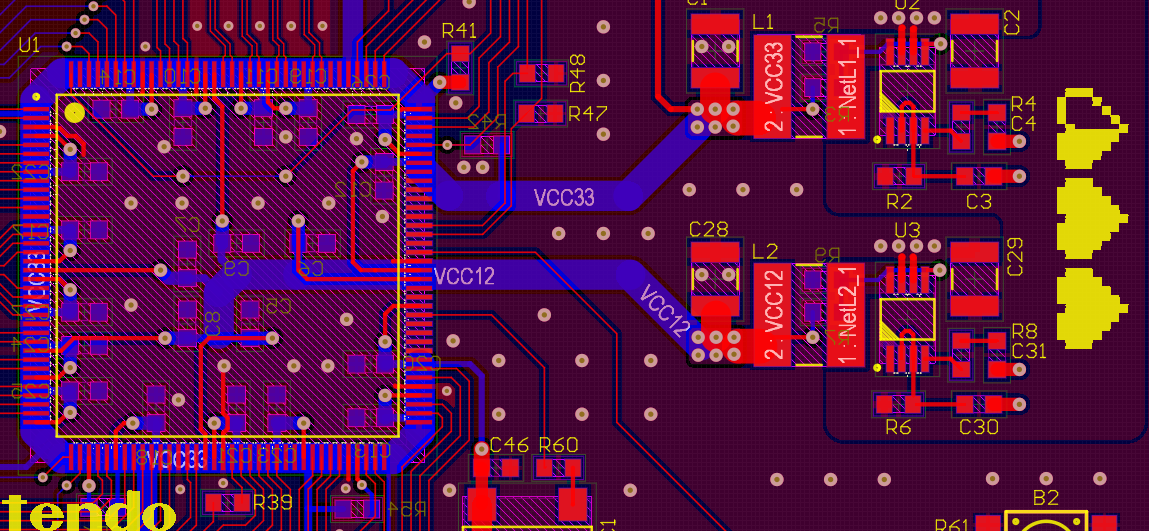
\includegraphics[width=150mm, keepaspectratio]{figures/FPGA-PSU-routing}
		\caption{FPGA tápellátásának kialakítása}
		\label{fig:FPGA-PSU-routing}
	\end{figure}
	
	A chip tápellátását \aref{fig:FPGA-PSU-routing}. ábrán láthatjuk, a kártya teljes tápellátását pedig \aref{sec:FPGA-nes-transparency}. függelékben figyelhetjük meg. 
	
	\subsection{FPGA NES 3D terve}
	
	A kártya tervezését követően az Altium designer lehetőséget nyújt a PCB 3D tervének megtekintéséhez (ez a komponensek elhelyezésénél, illetve nyák foglalatok tervezésénél is hasznos). Ez egy teljes képet nyújt a nyomtatott áramkör kialakításáról és jövőbeli kinézetéről. Az FPGA NES 3D tervét a következő \ref{fig:PCB-3D}. ábrán láthatjuk:  
	
	\begin{figure}[H]
		\centering
		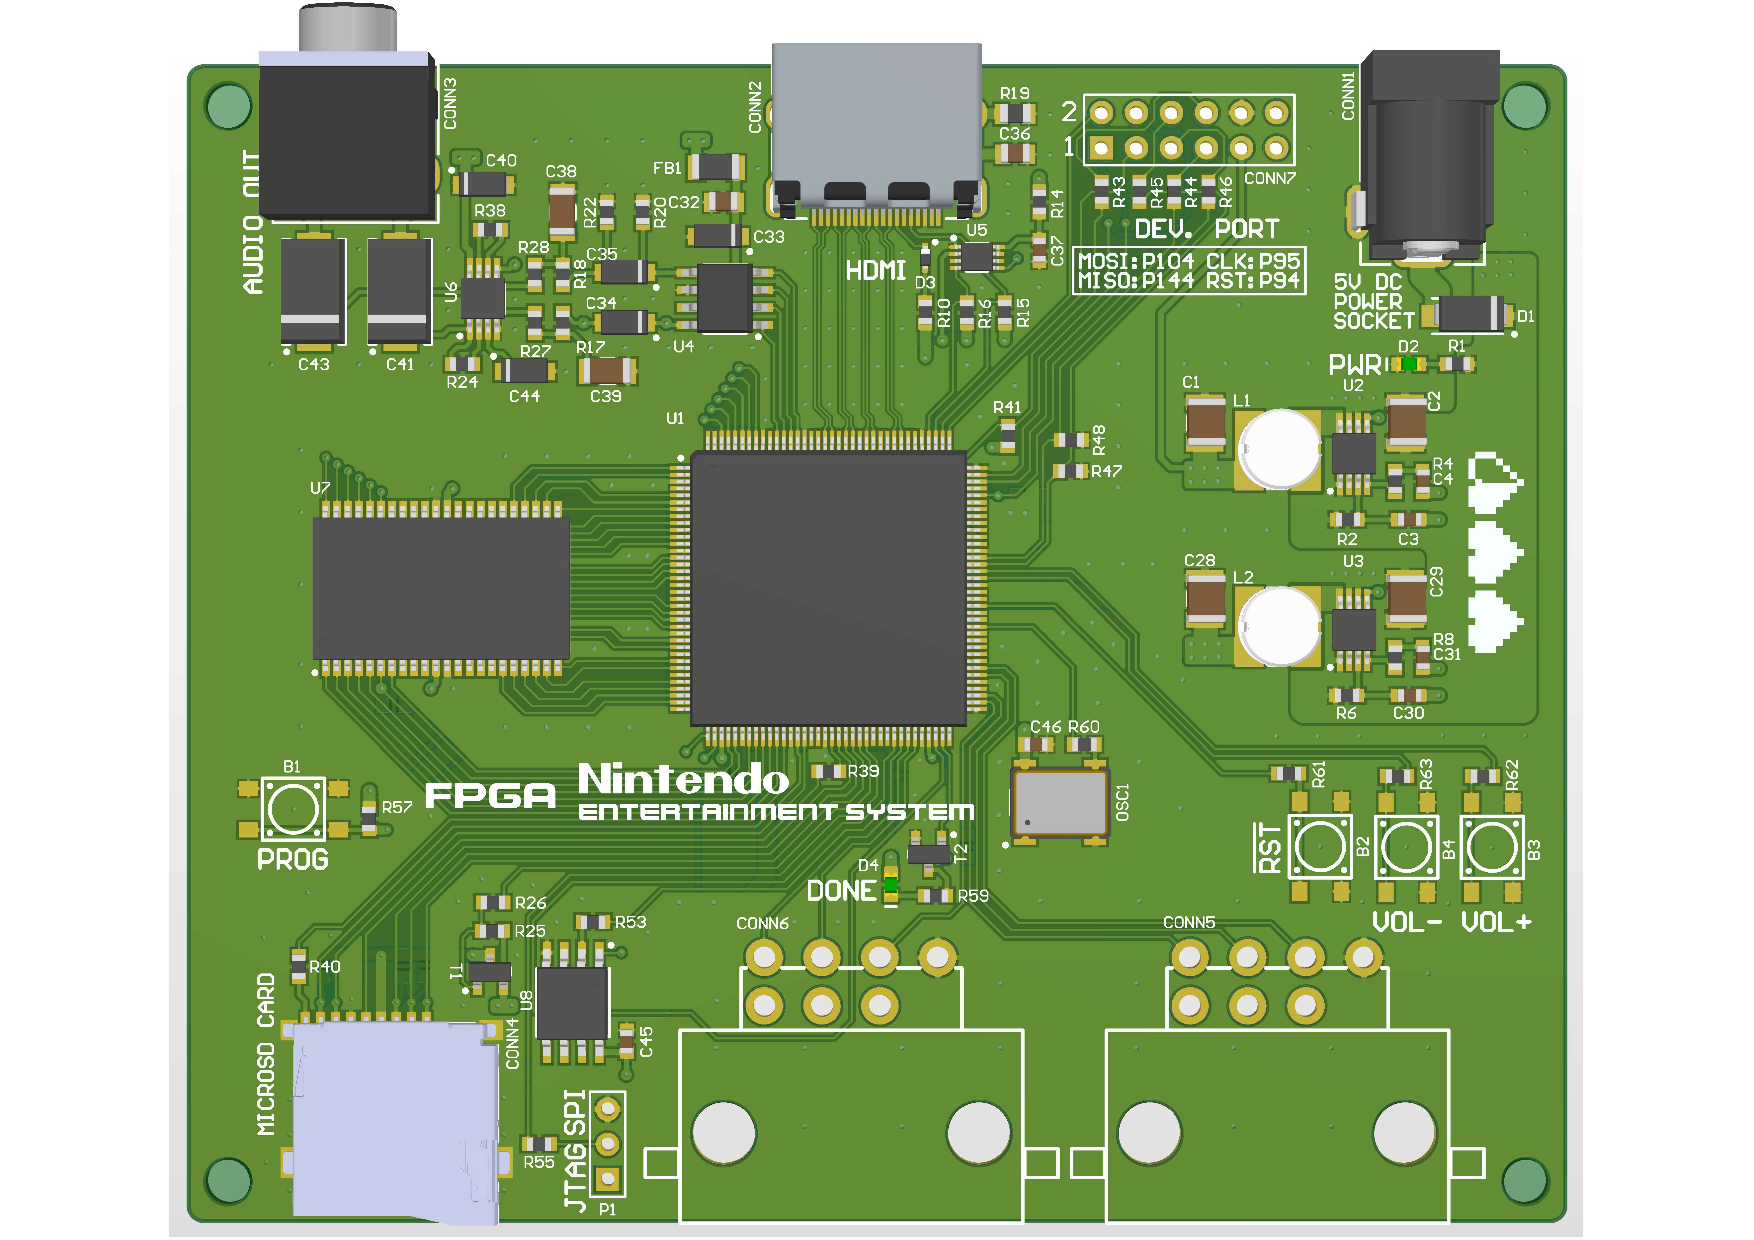
\includegraphics[width=100mm, keepaspectratio, angle=90]{figures/Top}
		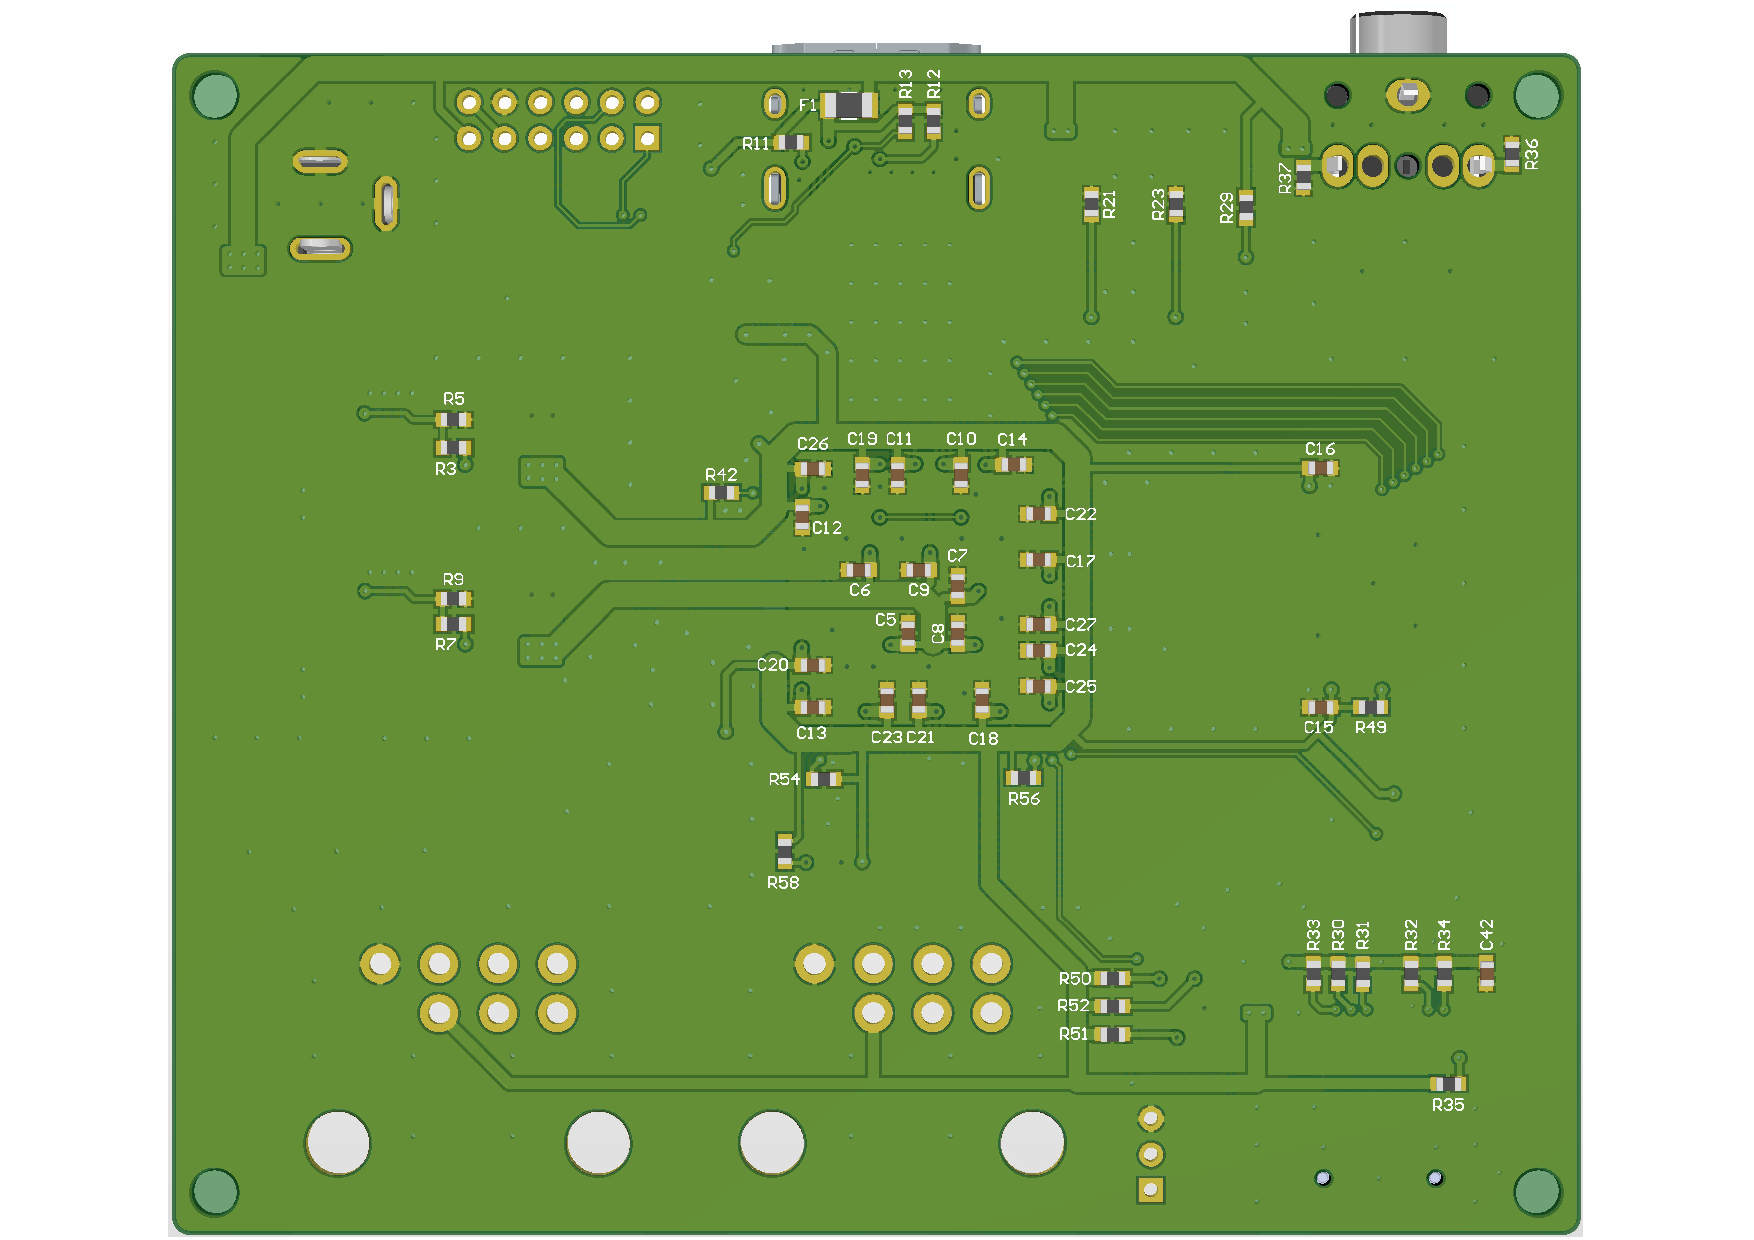
\includegraphics[width=100mm, keepaspectratio, angle=90]{figures/Bottom}
		\caption{3D PCB rajzolat} 
		\label{fig:PCB-3D}
	\end{figure}
	

	
	
	
	

